\documentclass[11pt]{report}

\usepackage{setspace}
\usepackage{fancyvrb}
\usepackage{graphicx}
\usepackage{geometry}
\usepackage{array}
\usepackage{hyperref}
\usepackage{multirow}

\setlength{\parindent}{4em}
\geometry{letterpaper, portrait, margin=0.75in}
\newcommand\tab[1][1cm]{\hspace*{#1}}

%%%Title Page%%%
\title{
	\begin{center}
		
\includegraphics[scale=0.5]{uga.PNG}\\
 	\end{center}
 	Project 3 Report
\bigbreak Performance Tuning of SQL Queries
}

\author{\textbf{Brandon Canaday, Jacob Ambrose, Zachary Davis}}

\date{\today}
%%%%%%%%%%%%

\begin{document}
\maketitle

\section*{Query Values}
	\begin{tabular}{l|l|l}
		\textbf{Name} & \textbf{Attribute} & \textbf{Value}\\
		\hline
		v1(Value1) & Student.id & 482081\\
		&&\\
		v2(Value2) & Student.id (Lower Bound) & 205181\\
		&&\\
		v3(Value3) & Student.id (Upper Bound) & 205000\\
		&&\\
		v4(Value4) & Course.crsCode & 166690\\
		&&\\
		v5(Value5) & Professor.name & name996317\\
		&&\\
		v6(Value6) & Department.id (Include) & 80028\\
		&&\\
		v7(Value7) & Department.id (Disclude) & 971318\\
		&&\\
		v8(Value8) & Department.id & 25784\\ 
	\end{tabular}

\section*{Before Optimization}
	\begin{flushleft}
		\begin{tabular}{m{15em}|m{27.5em}} 
			\textbf{Statement} & \textbf{Query} \\
			\hline
			\multirow{1}{15em}{1. List the name of the student with id equal to v1.} 
			& SELECT SQL\_NO\_CACHE s.name \\ 
			& FROM Student s \\ 
			& WHERE (s.id = 482081); \\
			&\\ 
			\multirow{1}{15em}{2. List the names of students with id in the range of v2 to v3 
			inclusively.} 
			& SELECT SQL\_NO\_CACHE s.name \\ 
			& FROM Student s \\ 
			& WHERE (s.id $<=$ 205181) AND (s.id $>=$ 205000); \\
			&\\
			&\\ 
			\multirow{1}{15em}{3. List the names of students who have taken course v4.} 
			& SELECT SQL\_NO\_CACHE s.name \\ 
			& FROM Transcript t \\ 
			& INNER JOIN Course c ON t.crsCode = c.crsCode \\
			& INNER JOIN Student s ON t.studId = s.id \\
			& WHERE c.crsCode = 166690; \\
			&\\ 
			\multirow{1}{15em}{4. List the names of students who have taken a course taught by 
			professor v5.} 
			& SELECT SQL\_NO\_CACHE s.name \\ 
			& FROM Transcript t \\ 
			& INNER JOIN Teaching te ON t.crsCode = te.crsCode \\
			& INNER JOIN Professor p ON te.profId = p.id \\
			& INNER JOIN Student s ON t.studId = s.id \\
			& WHERE p.name = 'name996317'; \\
		\end{tabular}
	\end{flushleft}

	\begin{flushleft}
		\begin{tabular}{m{15em}|m{27.5em}}
			\multirow{1}{15em}{5. List the names of students who have taken a course from 
			department v6, but not v7.} 
			& SELECT SQL\_NO\_CACHE s.name \\ 
			& FROM Transcript t \\ 
			& INNER JOIN Student s ON t.studId = s.id \\
			& INNER JOIN Course c ON t.crsCode = c.crsCode \\
			& WHERE (s.id IN  \\
			& \tab (SELECT s.id \\
			& \tab FROM Transcript t \\
			& \tab INNER JOIN Student s ON t.studId = s.id \\
			& \tab INNER JOIN Course c ON t.crsCode = c.crsCode \\
			& \tab INNER JOIN Department d ON c.deptId = d.id \\
			& \tab WHERE d.id = 80028 \\
			& \tab )) \\
			& \tab AND (s.id NOT IN \\
			& \tab (SELECT s.id \\
			& \tab FROM Transcript t \\
			& \tab INNER JOIN Student s ON t.studId = s.id \\
			& \tab INNER JOIN Course c ON t.crsCode = c.crsCode \\
			& \tab INNER JOIN Department d ON c.deptId = d.id \\
			& \tab WHERE d.id = 971318 \\
			& \tab)) \\
			& GROUP BY s.id; \\
			&\\ 
			&\\
			&\\
			\multirow{1}{15em}{6. List the names of students who have taken all courses offered 
			by department v8.} 
			& SELECT SQL\_NO\_CACHE s.name \\ 
			& FROM \\ 
			& \tab (SELECT ss.id, COUNT(*) AS courses \\
			& \tab FROM \\
			& \tab\tab (SELECT s.id, c.crsCode, d.id AS did \\
			& \tab\tab FROM Transcript t \\
			& \tab\tab INNER JOIN Student s ON t.studId = s.id \\
			& \tab\tab INNER JOIN Course c ON t.crsCode = c.crsCode \\
			& \tab\tab INNER JOIN Department d ON c.deptId = d.id \\
			& \tab\tab GROUP BY s.id, c.crsCode \\
			& \tab\tab ) AS ss \\
			& \tab WHERE ss.did = 25784 \\
			& \tab GROUP BY ss.id \\
			& \tab ) AS st \\
			& INNER JOIN Student s ON st.id = s.id \\
			& WHERE st.courses IN \\
			& \tab (SELECT COUNT(*) \\
			& \tab FROM Course c \\
			& \tab INNER JOIN Department d ON c.deptId = d.id \\
			& \tab WHERE d.id = 25784 \\
			& \tab ); \\
		\end{tabular}
	\end{flushleft}

\newpage

\section*{After Optimization}
	\begin{flushleft}
		\begin{tabular}{m{15em}|m{27.5em}} 
			\textbf{Statement} & \textbf{Query} \\
			\hline
			\multirow{1}{15em}{1. List the name of the student with id equal to v1.} 
			& SELECT name \\ 
			& FROM Student \\ 
			& WHERE id = 482081; \\
			&\\ 
			\multirow{1}{15em}{2. List the names of students with id in the range of v2 to v3 
			inclusively.} 
			& SELECT name \\ 
			& FROM Student \\ 
			& WHERE id BETWEEN 205000 AND 205181; \\
			&\\
			&\\ 
			\multirow{1}{15em}{3. List the names of students who have taken course v4.} 
			& SELECT s.name \\ 
			& FROM Transcript t \\ 
			& INNER JOIN Course c ON t.crsCode = c.crsCode \\
			& INNER JOIN Student s ON t.studId = s.id \\
			& WHERE c.crsCode = 166690; \\
			&\\ 
			\multirow{1}{15em}{4. List the names of students who have taken a course taught by 
			professor v5.} 
			& SELECT s.name \\ 
			& FROM Transcript t \\ 
			& INNER JOIN Student s ON t.studId = s.id \\
			& WHERE t.crsCode = 166690; \\
			\multirow{1}{15em}{5. List the names of students who have taken a course from 
			department v6, but not v7.} 
			& CREATE VIEW SinD AS SELECT s.id, d.id AS did \\ 
			& \tab FROM Transcript t \\ 
			& \tab INNER JOIN Student s ON t.studId = s.id \\
			& \tab INNER JOIN Course c ON t.crsCode = c.crsCode; \\
			& SELECT s.name \\
			& FROM Student s \\
			& WHERE s.id IN \\
			& \tab (SELECT id \\
			& \tab FROM SinD \\
			& \tab WHERE did = 80028 \\
			& \tab ) \\
			& \tab AND s.id NOT IN \\
			& \tab (SELECT id \\
			& \tab FROM SinD \\
			& \tab WHERE did = 971318 \\
			& \tab ); \\
		\end{tabular}
	\end{flushleft}

	\begin{flushleft}
		\begin{tabular}{m{15em}|m{27.5em}}
			\multirow{1}{15em}{6. List the names of students who have taken all courses offered 
			by department v8.} 
			& SELECT st.name \\ 
			& FROM \\ 
			& \tab (SELECT s.id, s.name, COUNT(DISTINCT c.crsCode) AS courses \\
			& \tab FROM Transcript t \\
			& \tab INNER JOIN Student s ON t.studId = s.id \\
			& \tab INNER JOIN Course c ON t.crsCode = c.crsCode \\
			& \tab WHERE c.deptid = 25784 \\
			& \tab GROUP BY s.id \\
			& \tab ) AS st \\
			& WHERE st.courses IN \\
			& \tab (SELECT COUNT(*) \\
			& \tab FROM Course c \\
			& \tab WHERE c.deptid = 25784 \\
			& \tab ); \\
		\end{tabular}
	\end{flushleft}

\section*{Explaining the Optimizations}
	\paragraph*{}
		In order to optimize our queries we first removed most of the parenthesis that were there for clarification. We then removed costly unnecessary JOIN operations using variables from other tables to complete the task. When running the Explain path we saw that in query 5 the same execution of steps run multiple times. So we created a view to simplify the task into 1 execution. For query 6, we moved our where condition to eliminate tuples before grouping them opposed to after. We then also created the table in a way that indexes the table for a significant time deduction. Below you can see the output of each of the queries. Even with the recommended amount of tuples the time was still too small. However, you can see in the explinations the significantly less operations nessesary in the optimized queries.

\newpage

\section*{Appendices}
	\paragraph*{Appendix A: Un-Optimized Queries}
		\begin{center}
			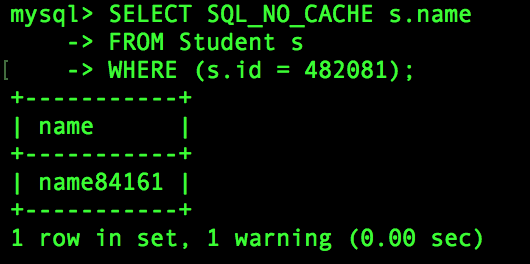
\includegraphics[scale=0.89]{b1.PNG}\\
			Figure 1.1: Query 1\\
			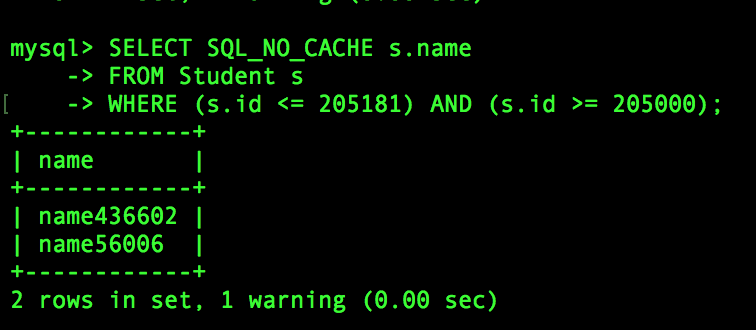
\includegraphics[scale=0.625]{b2.PNG}\\
			Figure 1.2: Query 2\\
			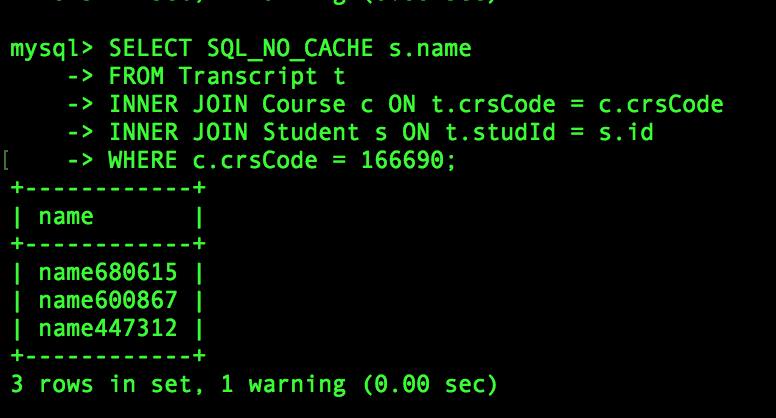
\includegraphics[scale=0.61]{b3.PNG}\\
			Figure 1.3: Query 3\\
			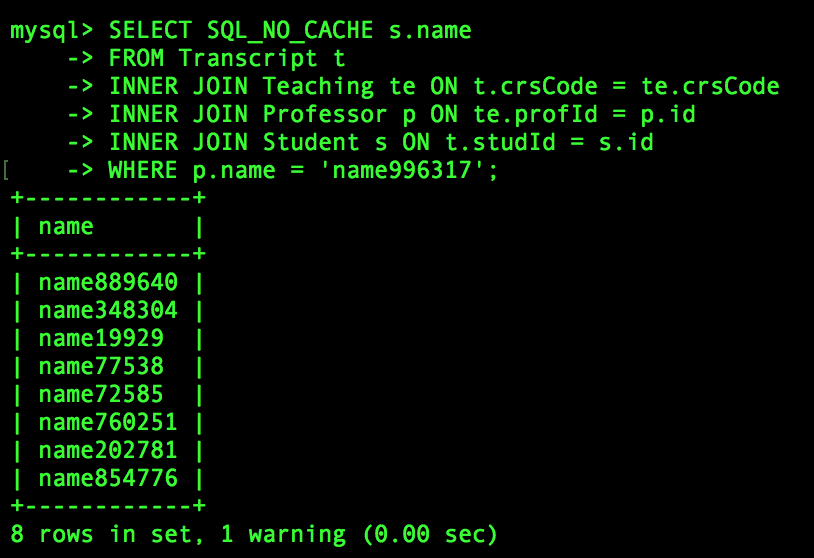
\includegraphics[scale=0.58]{b4.PNG}\\
			Figure 1.4: Query 4\\
			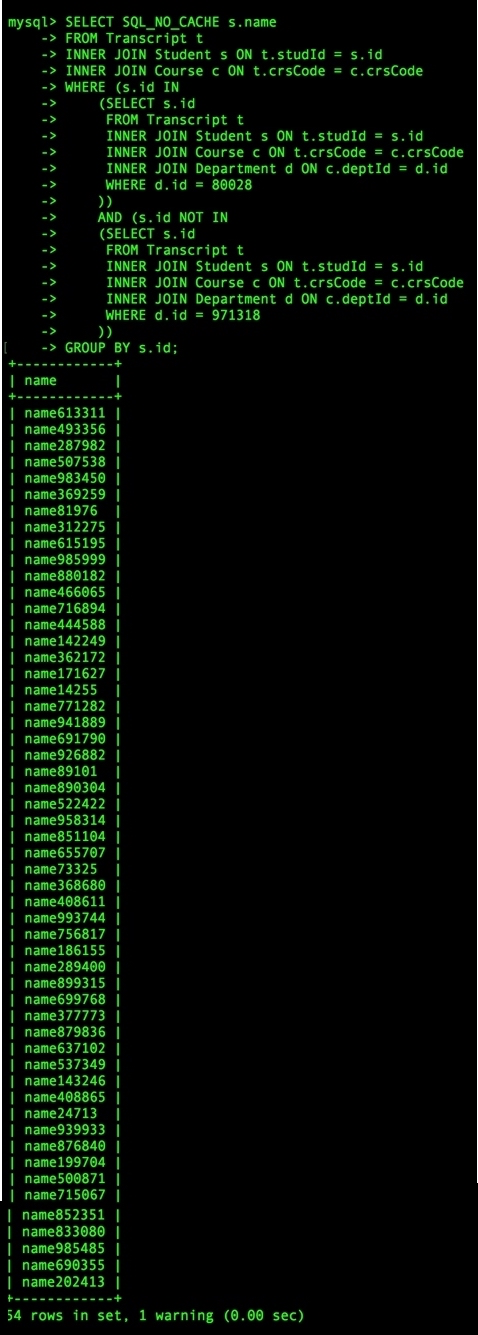
\includegraphics[scale=0.5]{b5.PNG}\\
			Figure 1.5: Query 5\\
			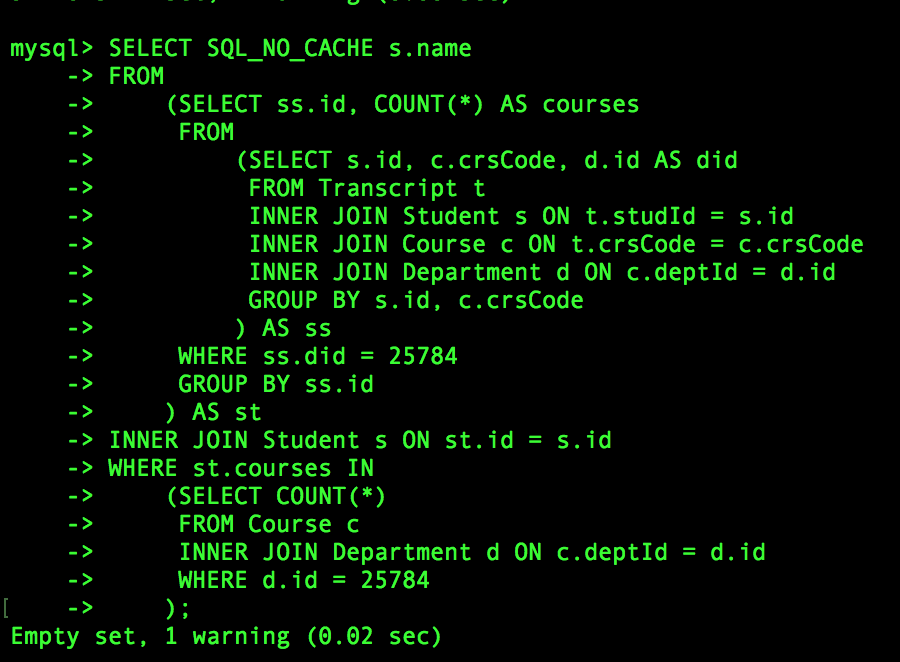
\includegraphics[scale=0.55]{b6.PNG}\\
			Figure 1.6: Query 6\\
		\end{center}
	\paragraph*{Appendix B: Un-Optimized Queries w/ Explination}
		\begin{center}
			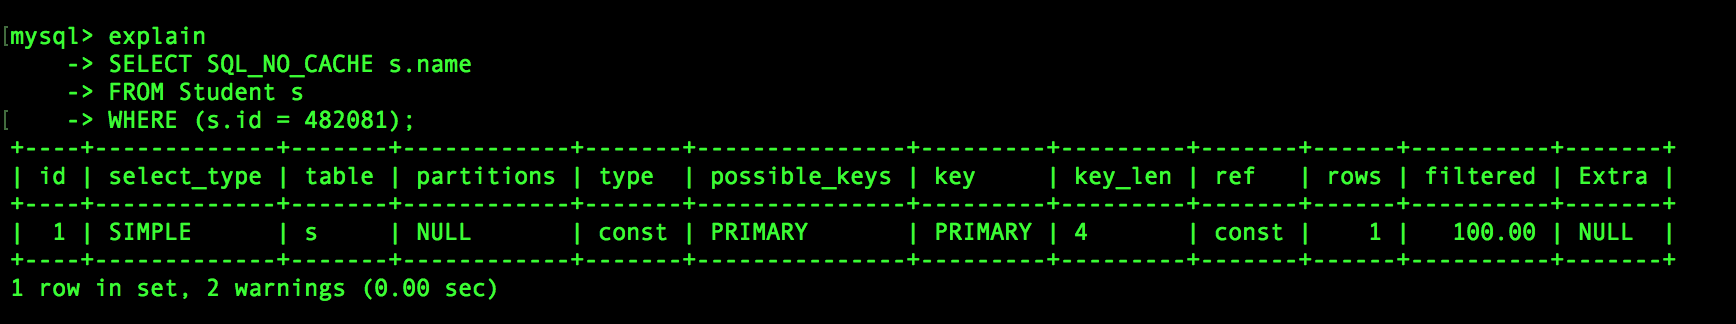
\includegraphics[scale=0.5]{Eb1.PNG}\\
			Figure 2.1: Query 1\\
			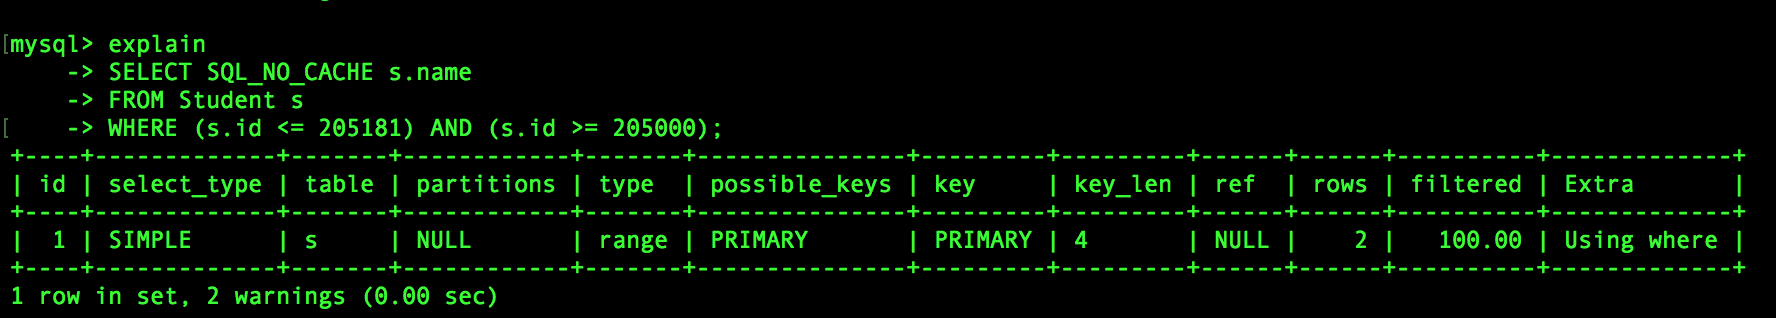
\includegraphics[scale=0.49]{Eb2.PNG}\\
			Figure 2.2: Query 2\\
			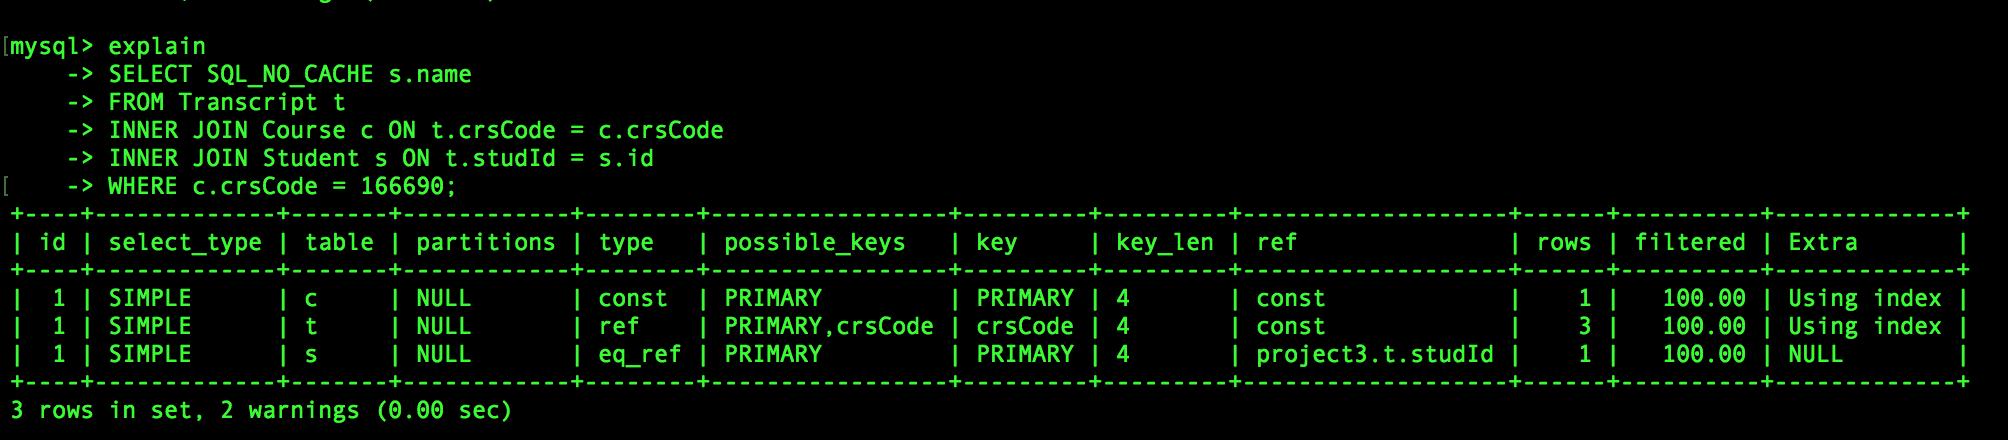
\includegraphics[scale=0.434]{Eb3.PNG}\\
			Figure 2.3: Query 3\\
			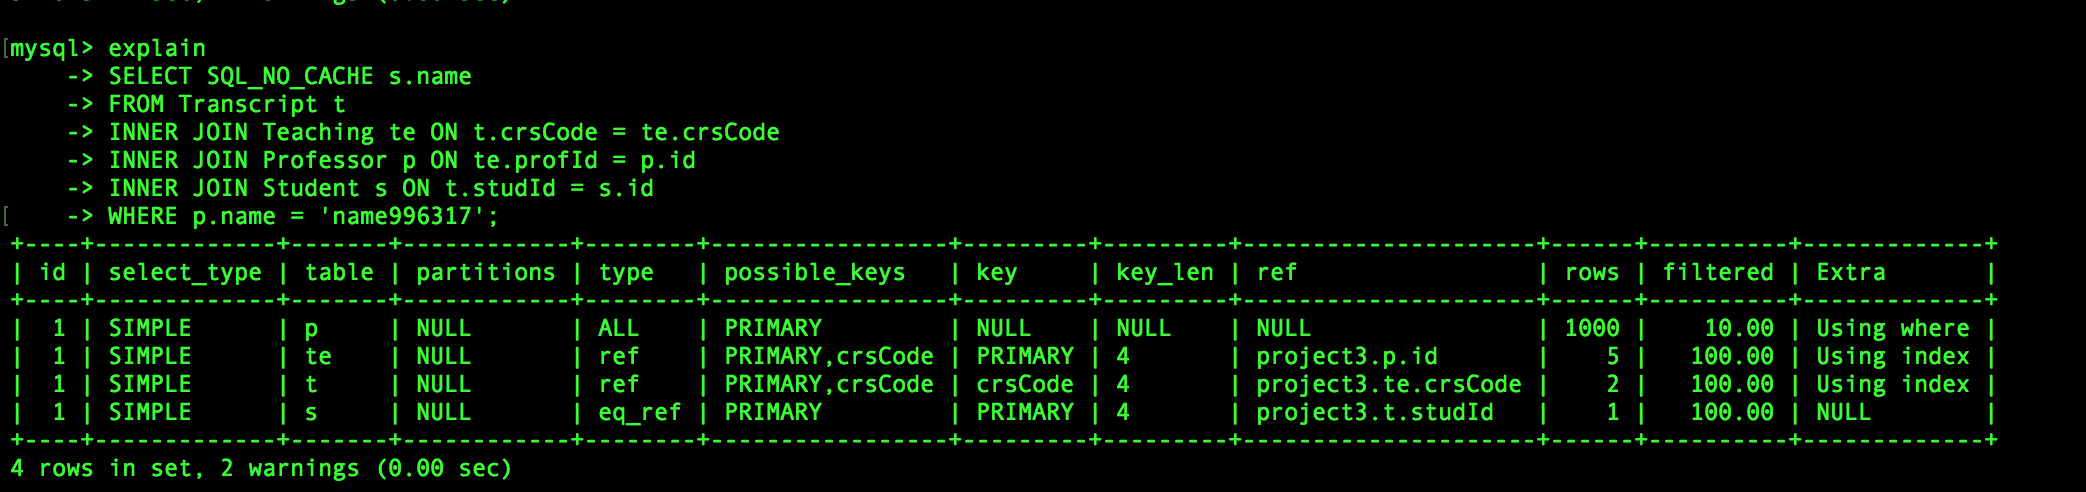
\includegraphics[scale=0.42]{Eb4.PNG}\\
			Figure 2.4: Query 4\\
			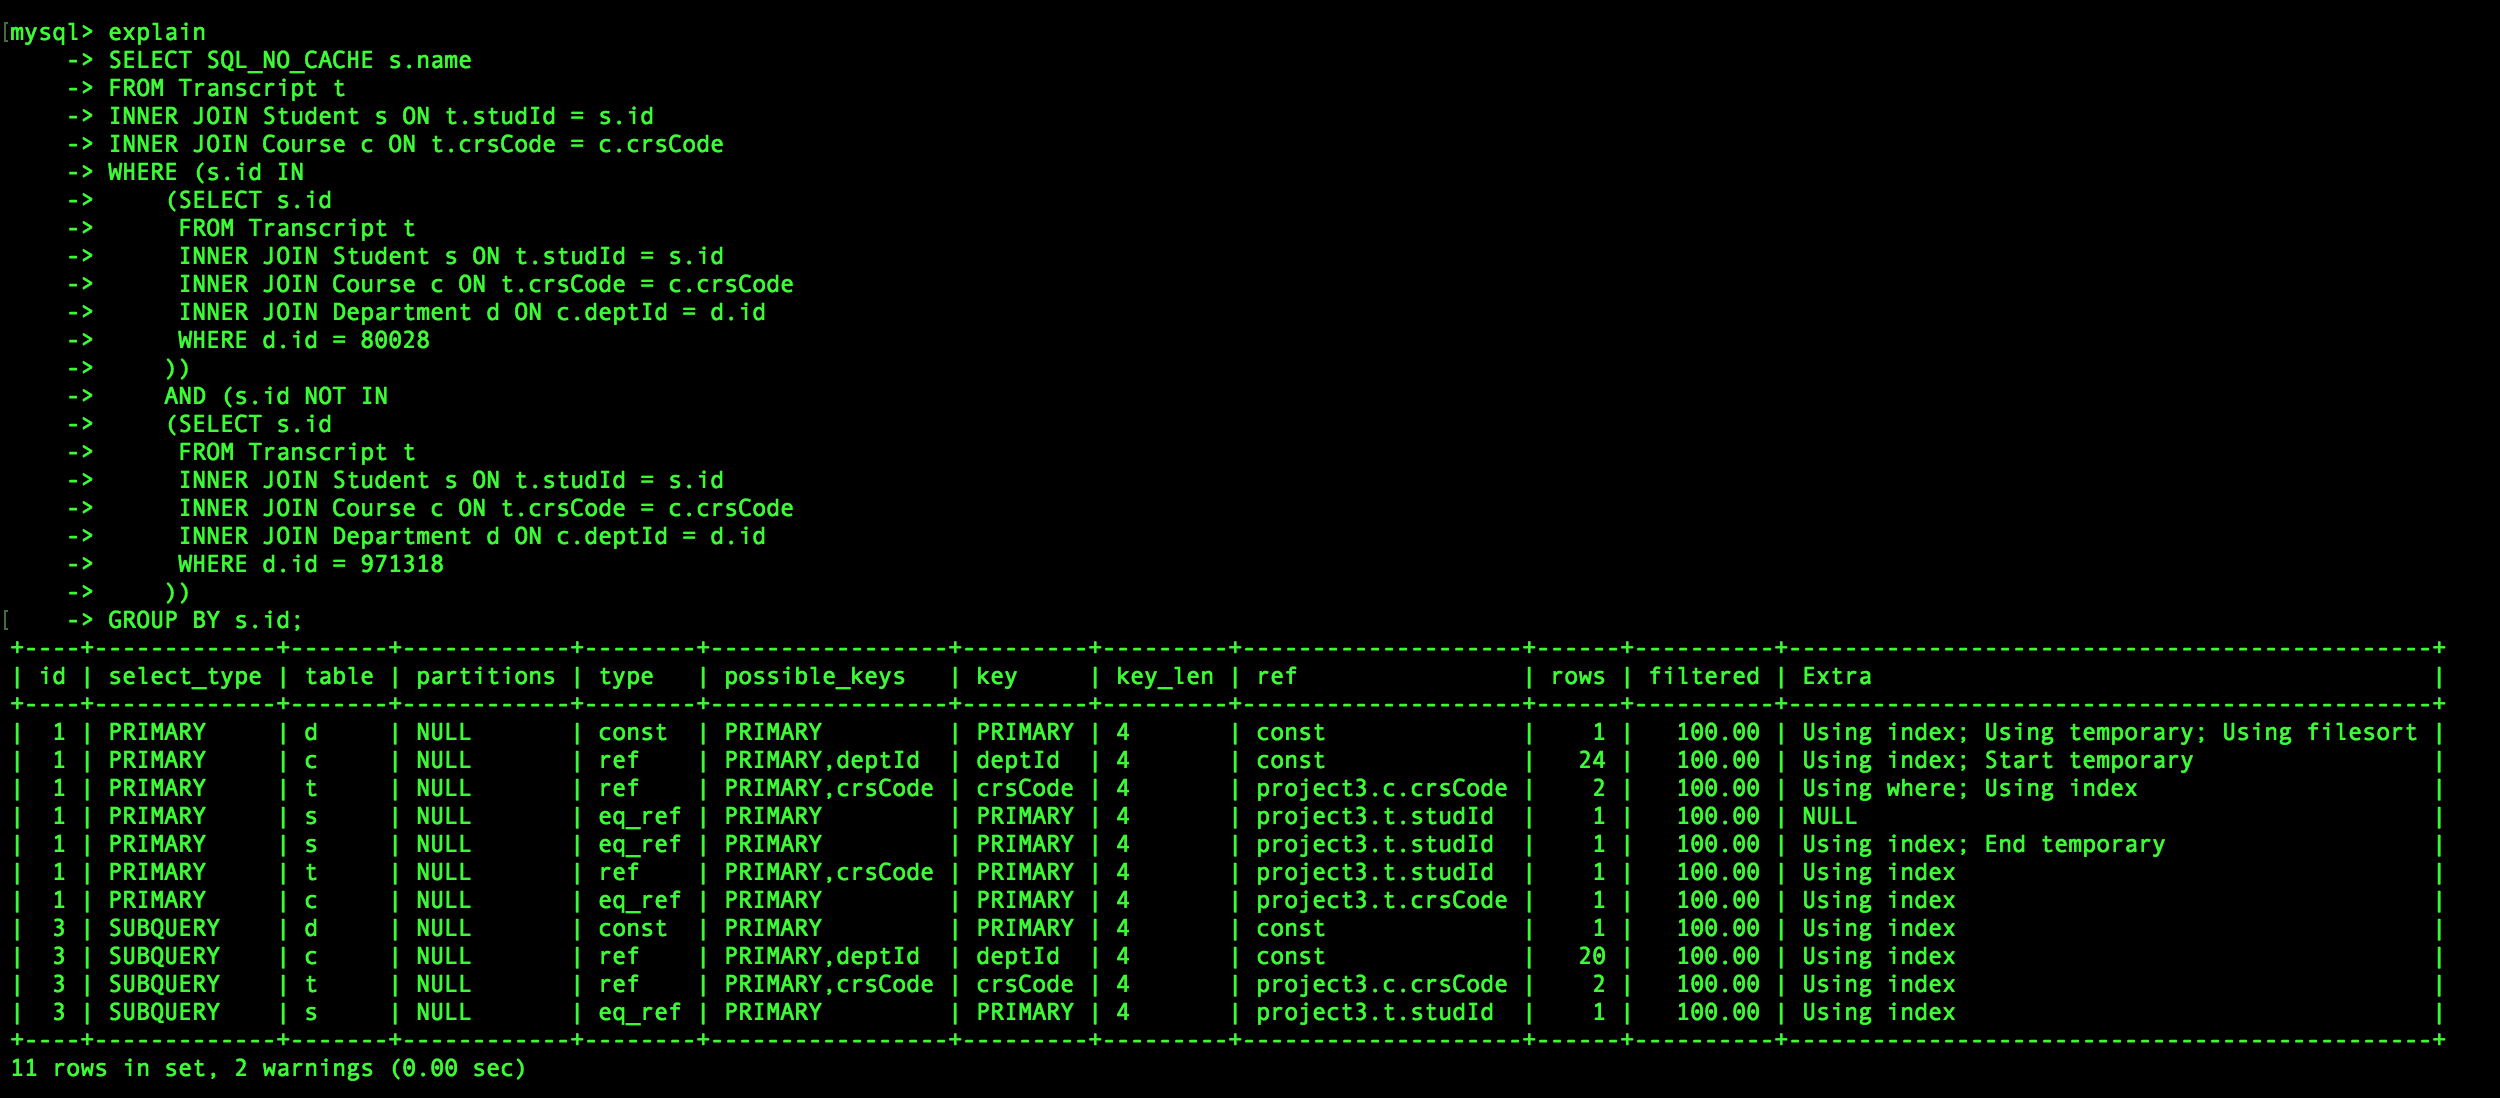
\includegraphics[scale=0.355]{Eb5.PNG}\\
			Figure 2.5: Query 5\\
			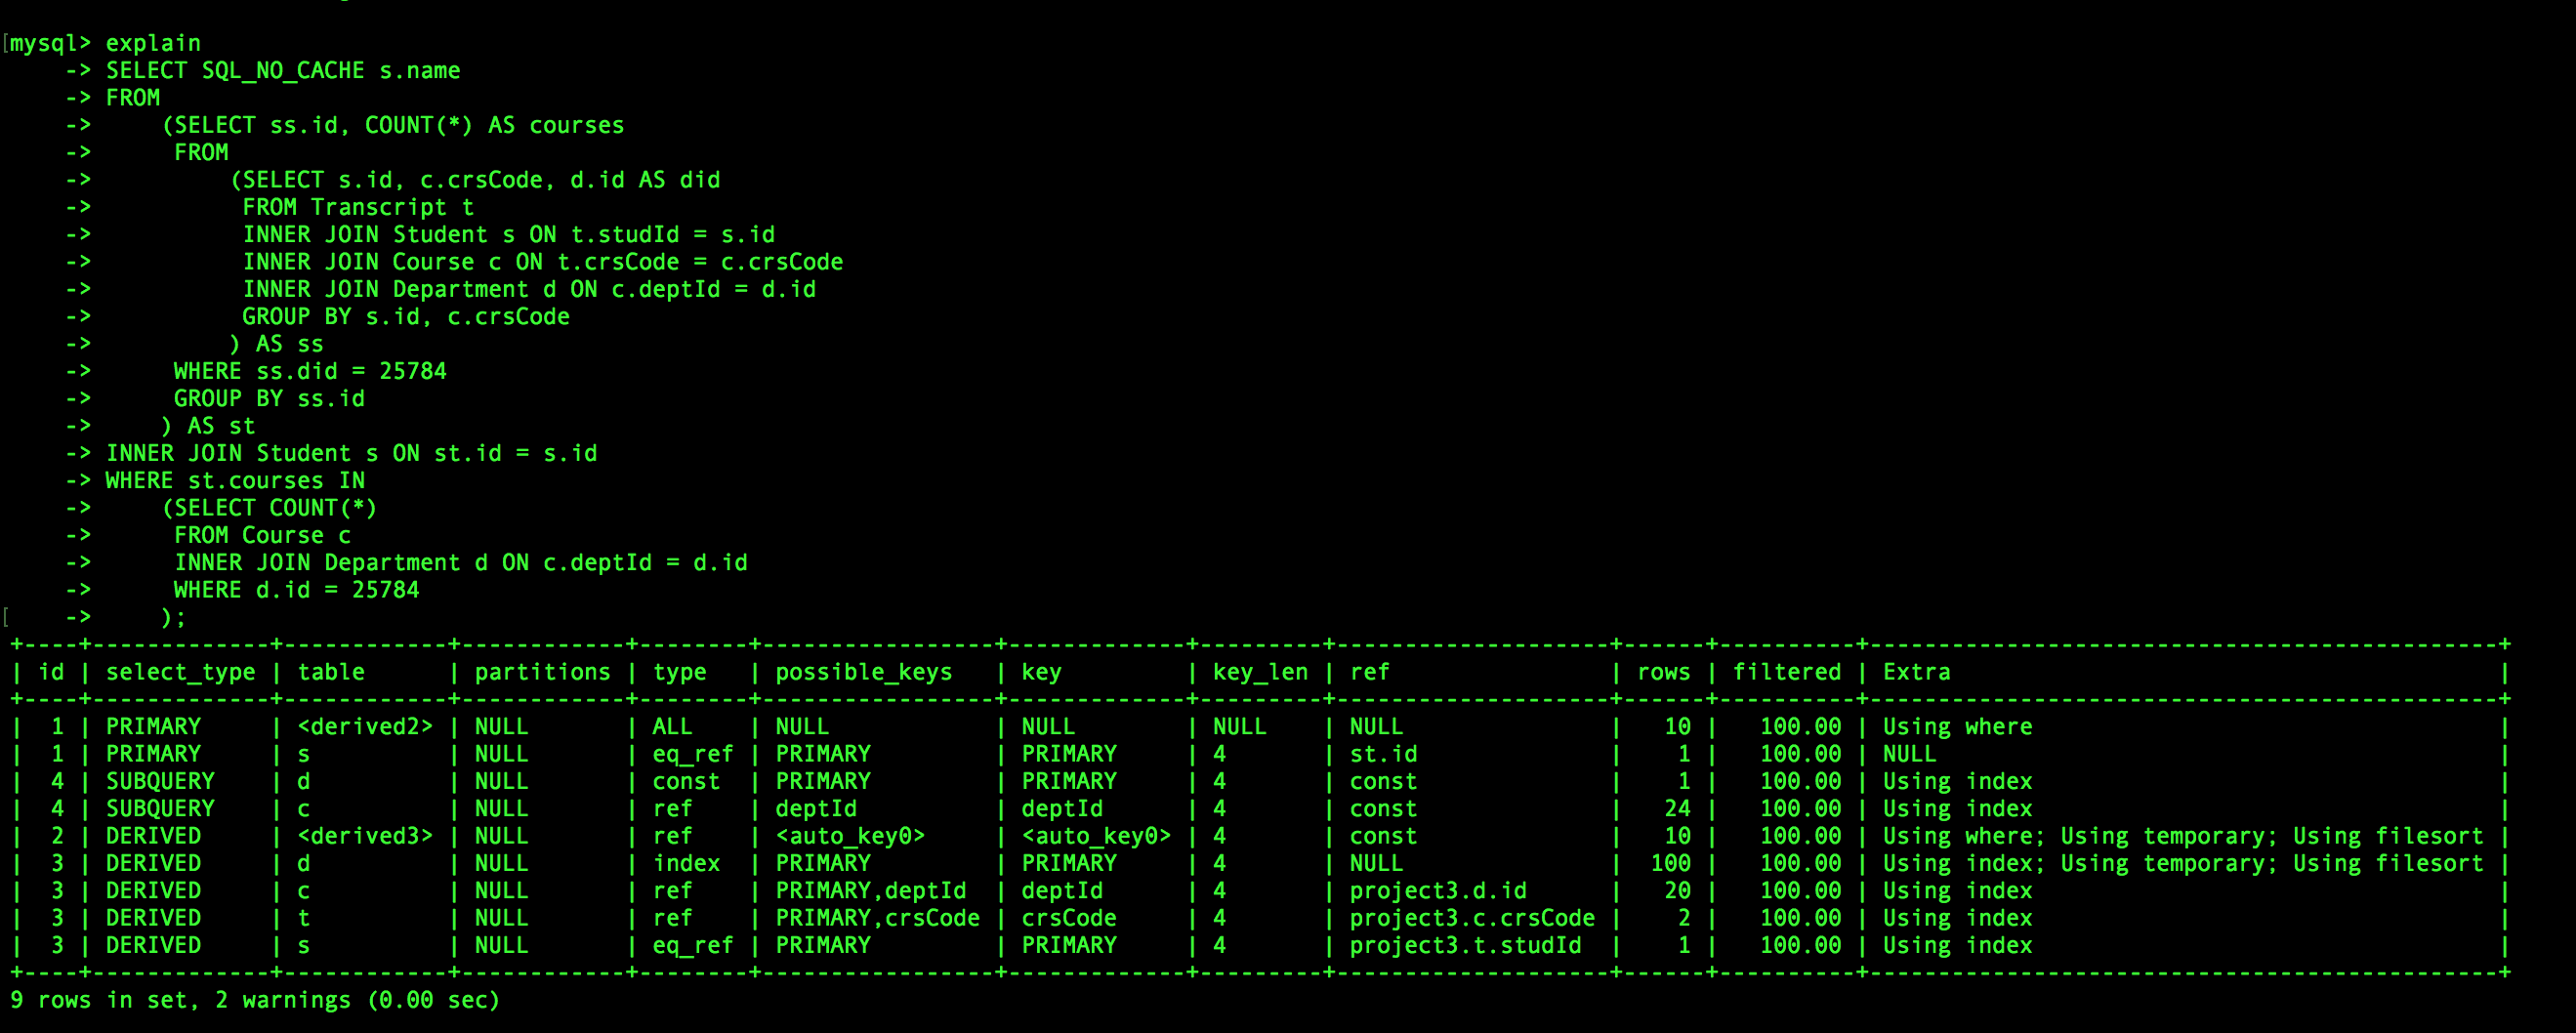
\includegraphics[scale=0.336]{Eb6.PNG}\\
			Figure 2.6: Query 6\\
		\end{center}
	\paragraph*{Appendix C: Optimized Queries}
		\begin{center}
			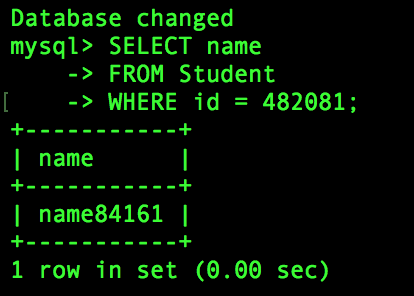
\includegraphics[scale=0.8]{a1.PNG}\\
			Figure 3.1: Query 1\\
			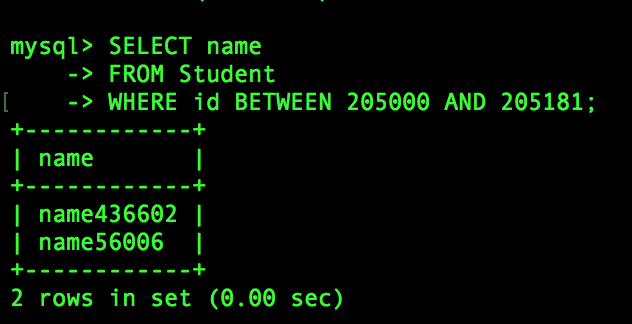
\includegraphics[scale=0.53]{a2.PNG}\\
			Figure 3.2: Query 2\\
			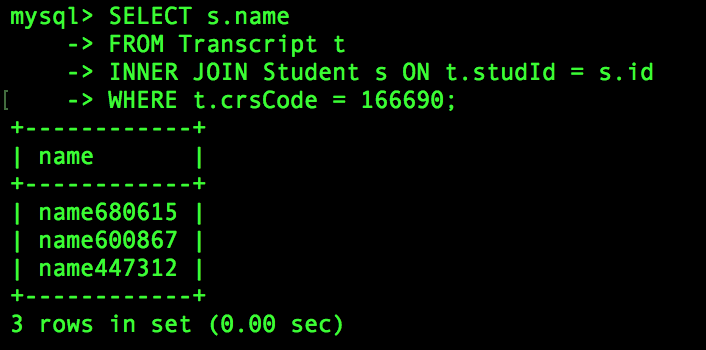
\includegraphics[scale=0.55]{a3.PNG}\\
			Figure 3.3: Query 3\\
			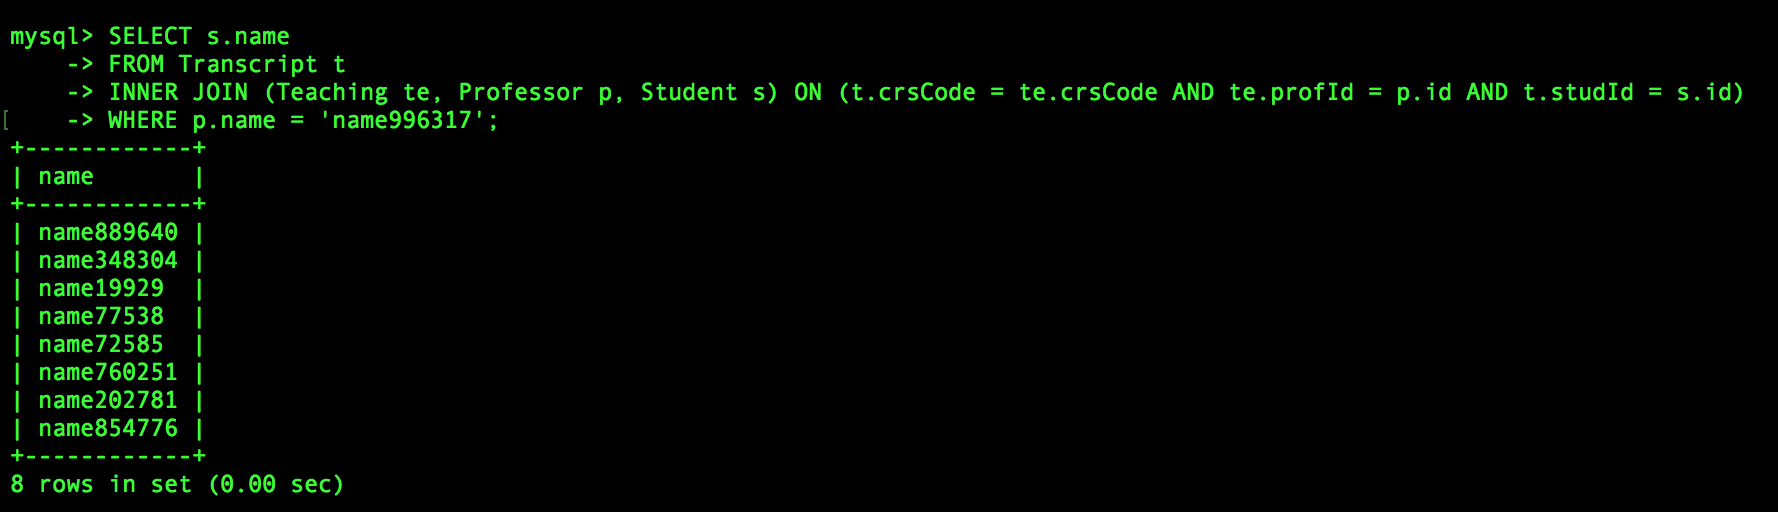
\includegraphics[scale=0.48]{a4.PNG}\\
			Figure 3.4: Query 4\\
			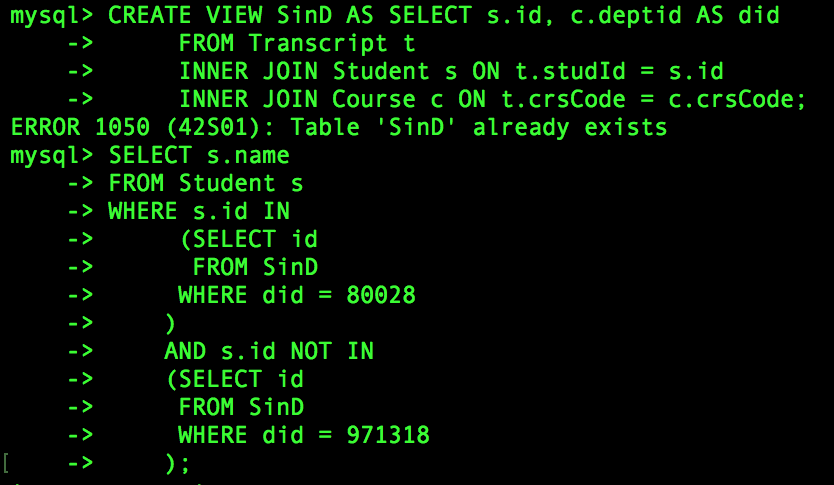
\includegraphics[scale=0.35]{a5-1.PNG}\\
			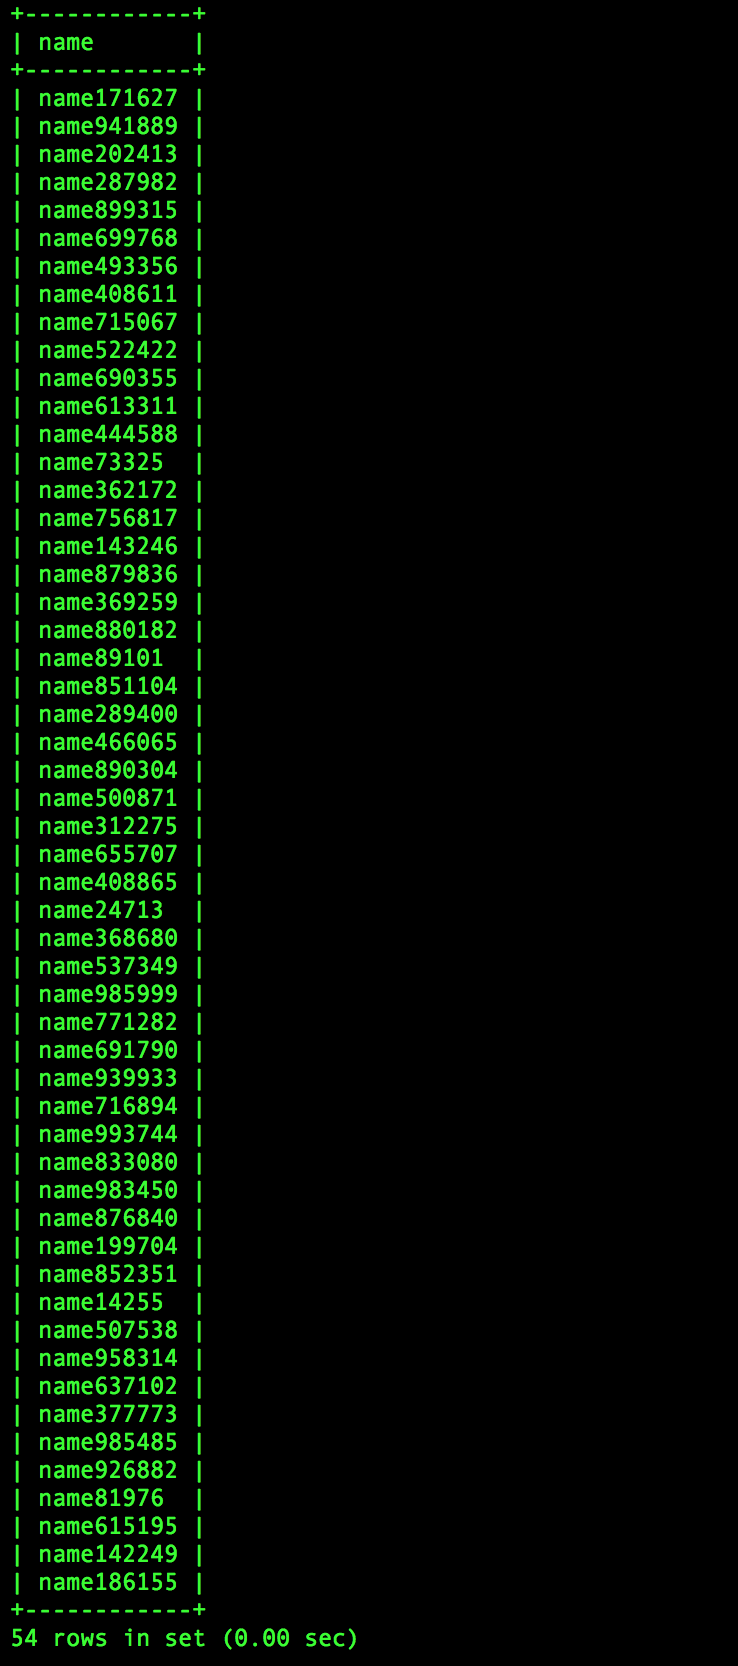
\includegraphics[scale=0.395]{a5-2.PNG}\\
			Figure 3.5: Query 5\\
			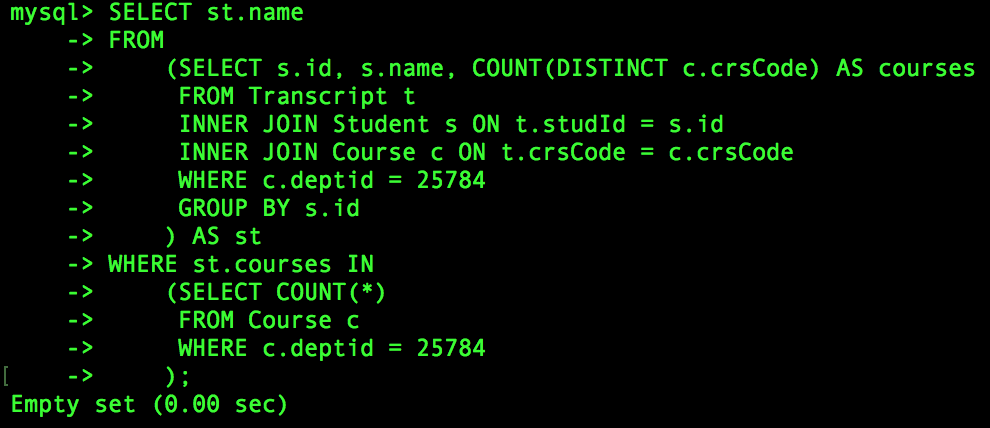
\includegraphics[scale=0.336]{a6.PNG}\\
			Figure 3.6: Query 6\\
		\end{center}
	\paragraph*{Appendix D: Optimized Queries w/ Explination}
		\begin{center}
			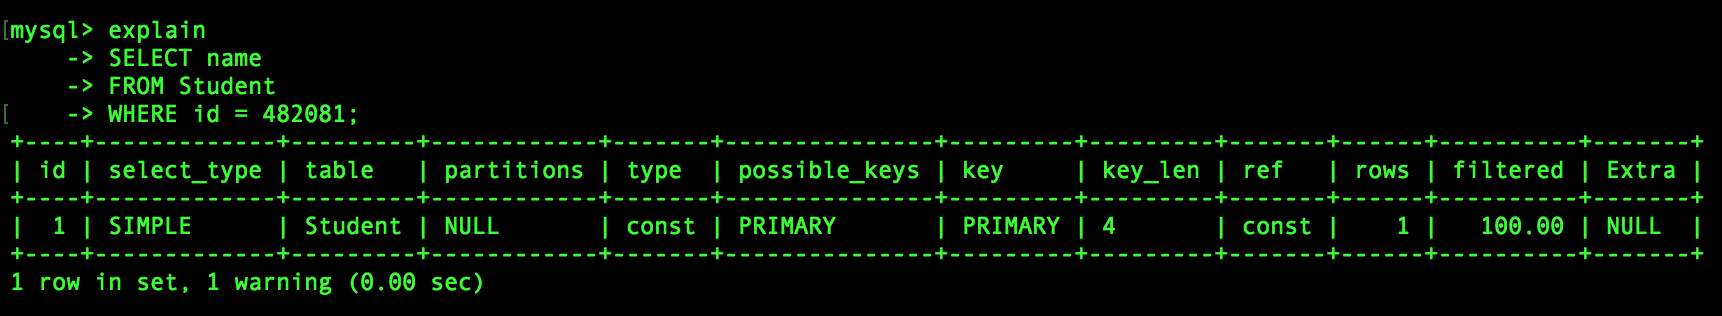
\includegraphics[scale=0.5]{Ea1.PNG}\\
			Figure 4.1: Query 1\\
			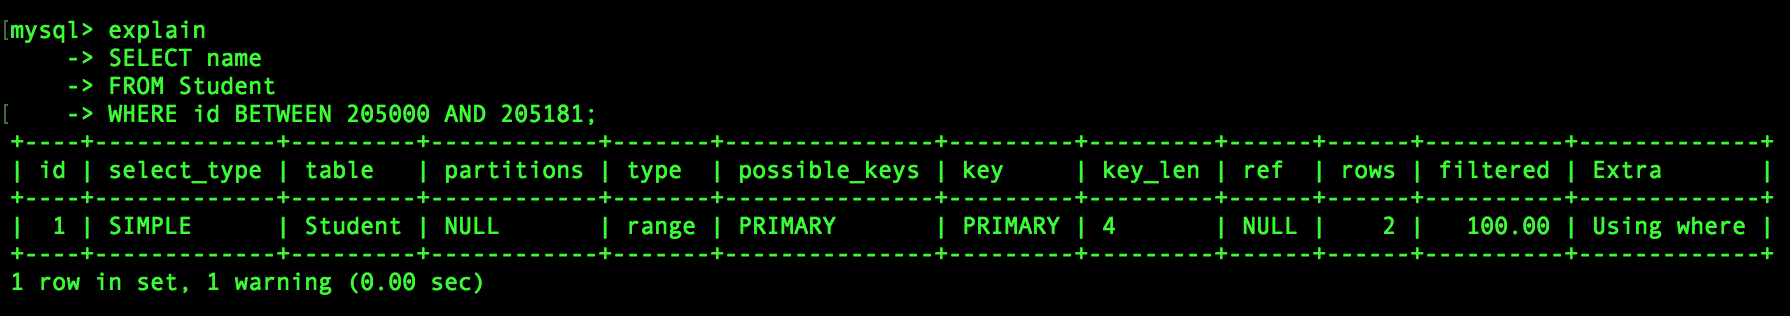
\includegraphics[scale=0.485]{Ea2.PNG}\\
			Figure 4.2: Query 2\\
			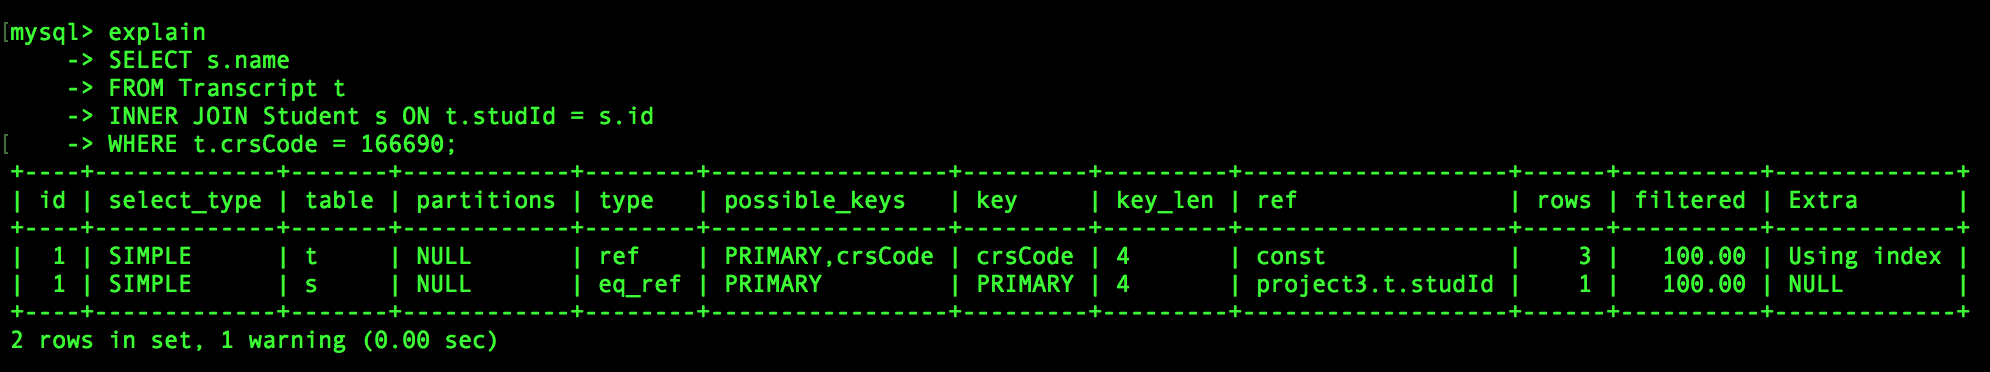
\includegraphics[scale=0.438]{Ea3.PNG}\\
			Figure 4.3: Query 3\\
			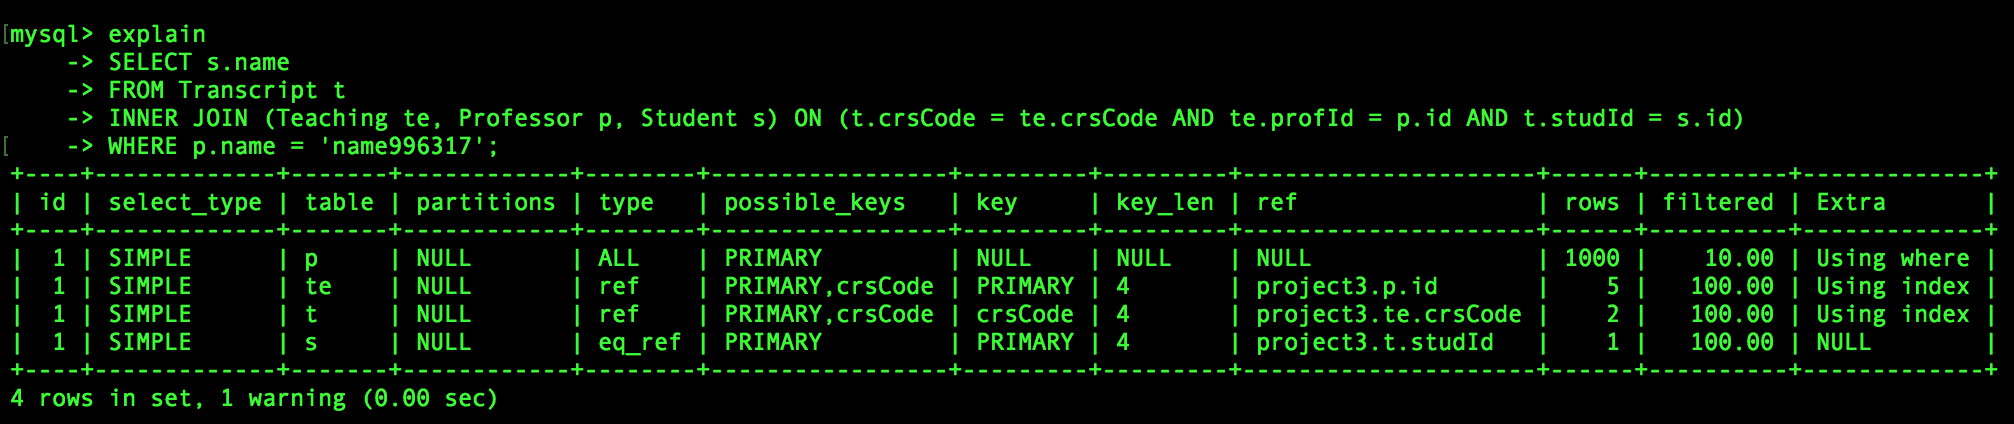
\includegraphics[scale=0.435]{Ea4.PNG}\\
			Figure 4.4: Query 4\\
			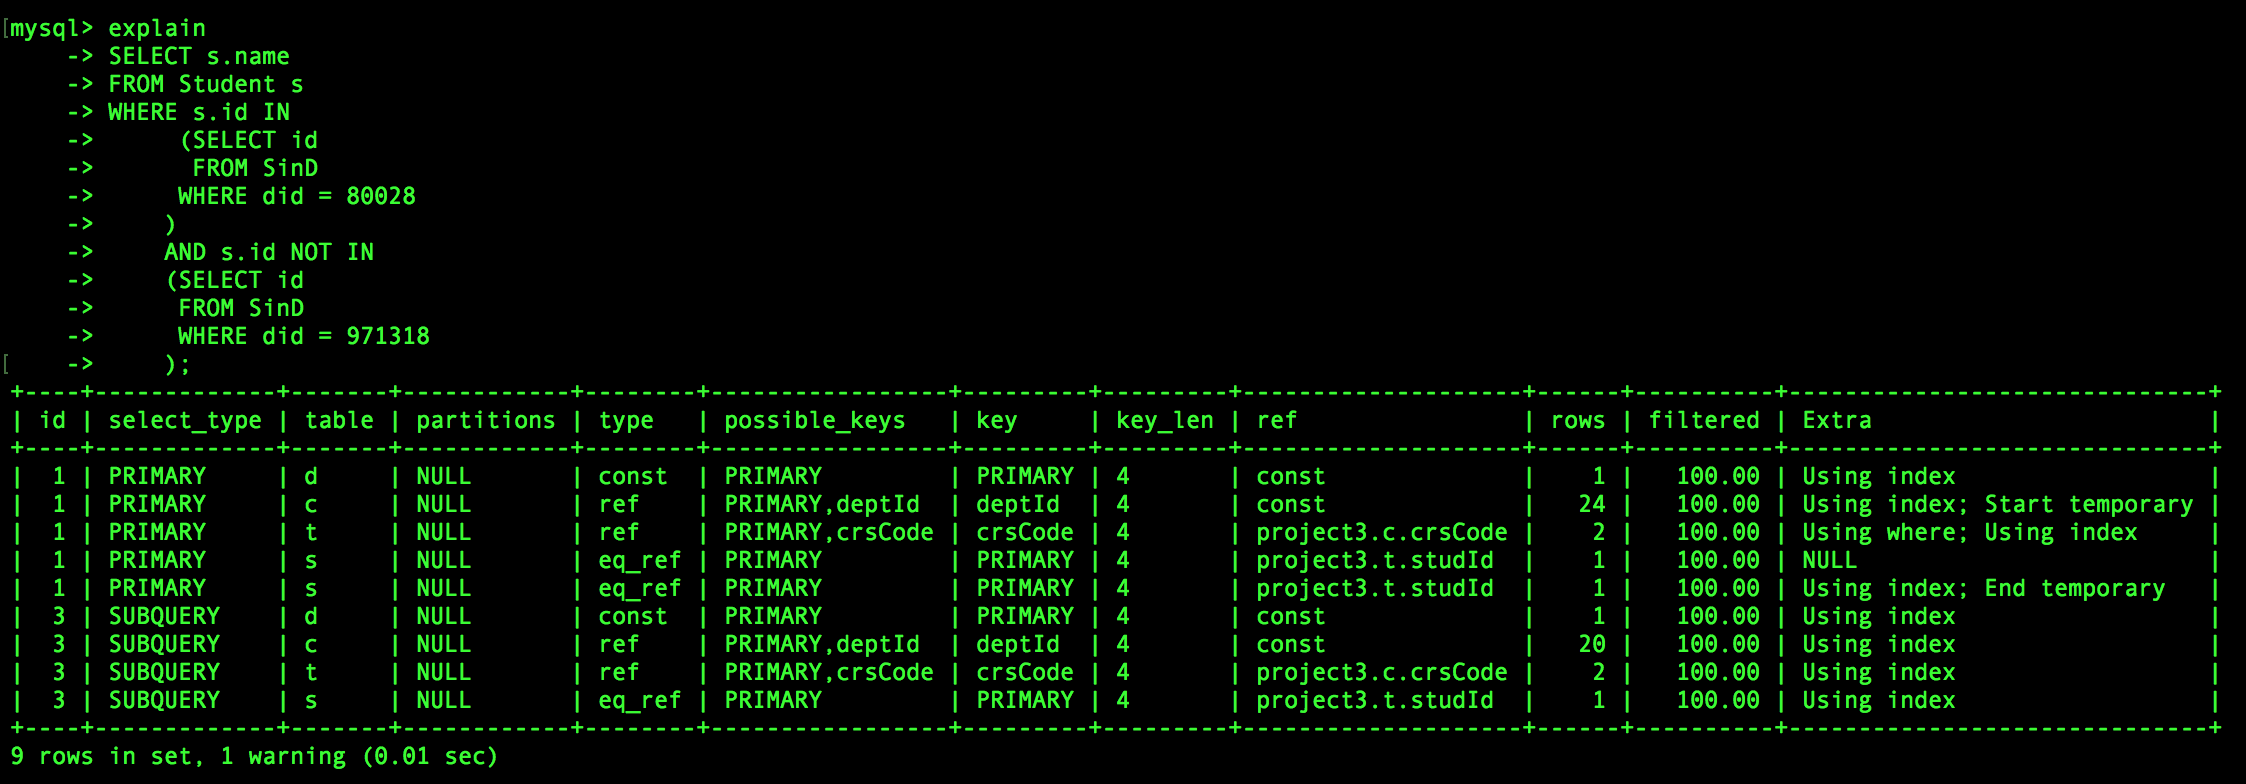
\includegraphics[scale=0.388]{Ea5.PNG}\\
			Figure 4.5: Query 5\\
			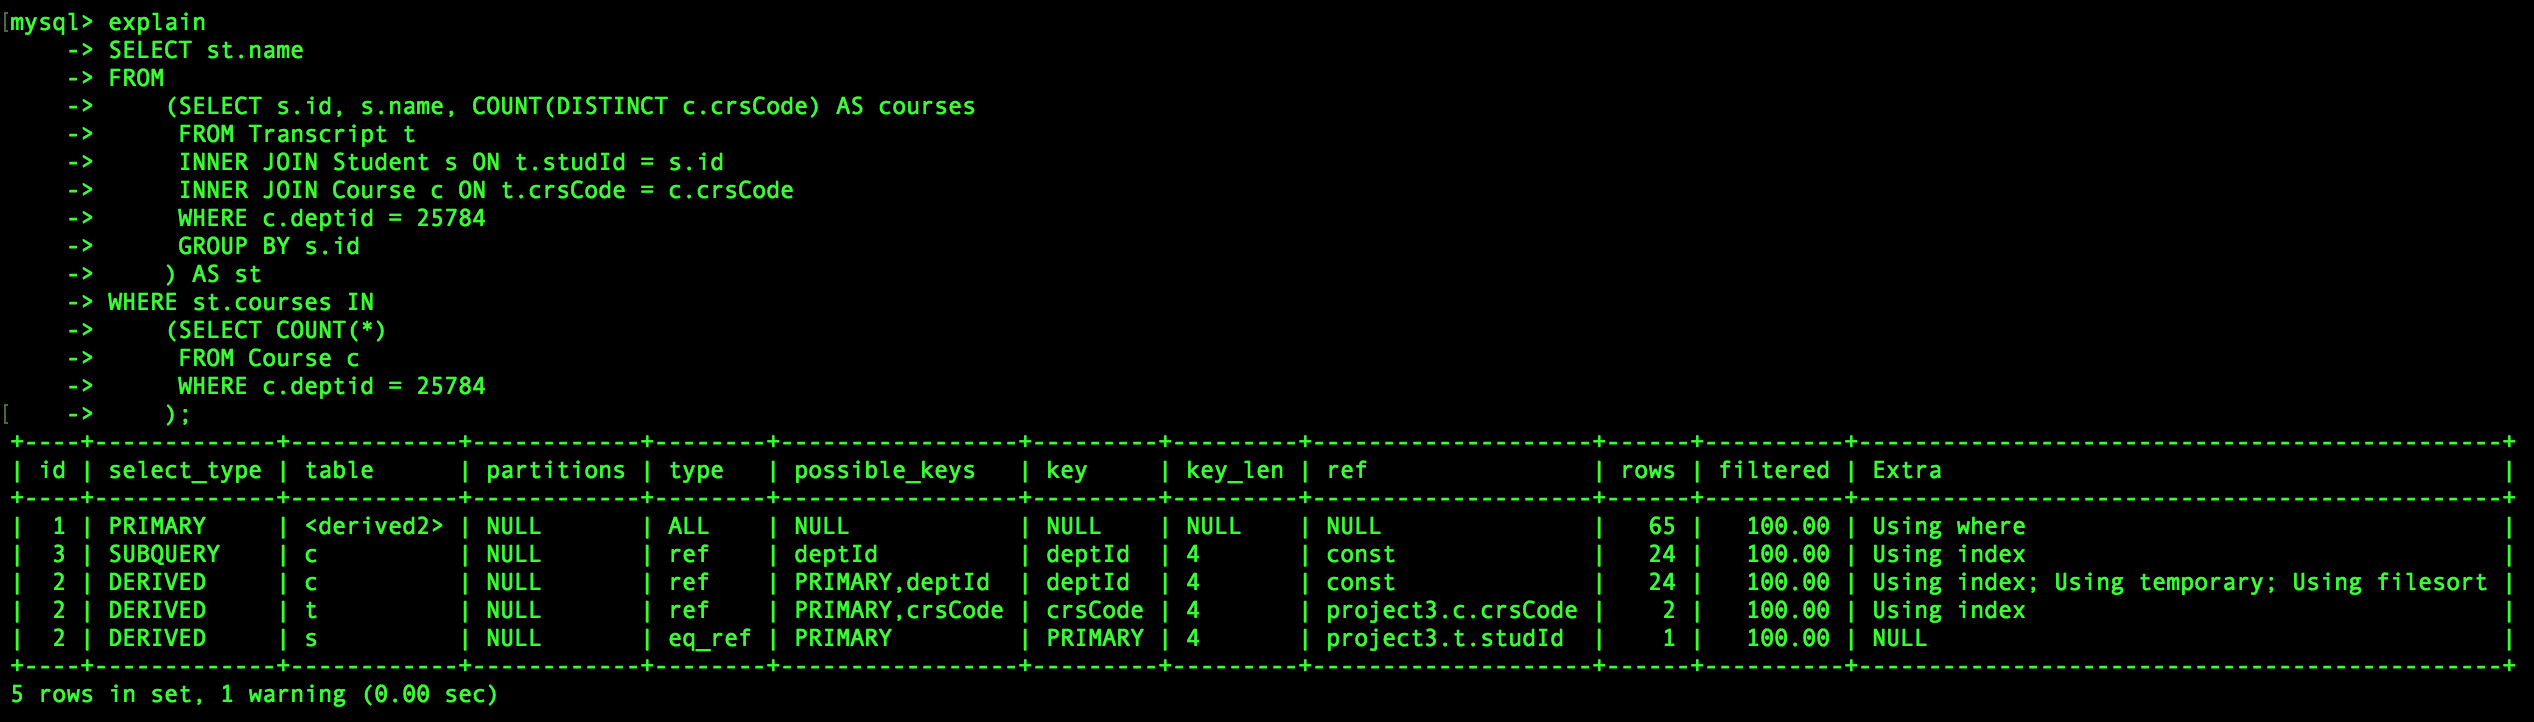
\includegraphics[scale=0.35]{Ea6.PNG}\\
			Figure 4.6: Query 6\\
		\end{center}	
\end{document}